%%%%%%%%%%%%%%%%%%%%%%%%%%%%%%%%%%%%%%%%%
% University Assignment Title Page
% LaTeX Template
% Version 1.0 (27/12/12)
%
% This template has been downloaded from:
% http://www.LaTeXTemplates.com
%
% Original author:
% WikiBooks (http://en.wikibooks.org/wiki/LaTeX/Title_Creation)
%
% License:
% CC BY-NC-SA 3.0 (http://creativecommons.org/licenses/by-nc-sa/3.0/)
%
% Instructions for using this template:
% This title page is capable of being compiled as is. This is not useful for
% including it in another document. To do this, you have two options:
%
% 1) Copy/paste everything between \begin{document} and \end{document}
% starting at \begin{titlepage} and paste this into another LaTeX file where you
% want your title page.
% OR
% 2) Remove everything outside the \begin{titlepage} and \end{titlepage} and
% move this file to the same directory as the LaTeX file you wish to add it to.
% Then add \input{./title_page_1.tex} to your LaTeX file where you want your
% title page.
%
%%%%%%%%%%%%%%%%%%%%%%%%%%%%%%%%%%%%%%%%%
%\title{Title page with logo}
%----------------------------------------------------------------------------------------
%	PACKAGES AND OTHER DOCUMENT CONFIGURATIONS
%----------------------------------------------------------------------------------------

\documentclass[12pt]{article}
\usepackage[french]{babel}
\usepackage[utf8x]{inputenc}
\usepackage{amsmath}
\usepackage{graphicx}
\usepackage[colorinlistoftodos]{todonotes}
\usepackage{listings}
\usepackage{float}
\usepackage[justification=centering]{caption}
\usepackage[toc,page]{appendix}
\usepackage{url}
\usepackage{pgfplots}

\setlength{\parskip}{0.2cm}%

\begin{document}

\begin{titlepage}

\newcommand{\HRule}{\rule{\linewidth}{0.5mm}} % Defines a new command for the horizontal lines, change thickness here

\center % Center everything on the page

%----------------------------------------------------------------------------------------
%	HEADING SECTIONS
%----------------------------------------------------------------------------------------

\textsc{\LARGE SORBONNE UNIVERSITE}\\[1.5cm] % Name of your university/college
\textsc{\Large Projet SAR}\\[0.5cm] % Major heading such as course name
\textsc{\large }\\[0.5cm] % Minor heading such as course title

%----------------------------------------------------------------------------------------
%	TITLE SECTION
%----------------------------------------------------------------------------------------

\HRule \\[0.4cm]
{ \huge \bfseries Ordonnancement de processus avec prise en compte de la synchronisation}\\[0.4cm] % Title of your document
\HRule \\[1.5cm]

%----------------------------------------------------------------------------------------
%	AUTHOR SECTION
%----------------------------------------------------------------------------------------

\begin{minipage}{0.4\textwidth}
\begin{flushleft} \large
\emph{Auteurs:}\\
Pierre-Loup \textsc{Gosse}\\
Salim Toufik \textsc{Nedjam}
\end{flushleft}
\end{minipage}
~
\begin{minipage}{0.4\textwidth}
\begin{flushright} \large
\emph{Encadrants:} \\
Redha \textsc{Gouicem}\\
Julien \textsc{Sopena}
\end{flushright}
\end{minipage}\\[2cm]

% If you don't want a supervisor, uncomment the two lines below and remove the section above
%\Large \emph{Author:}\\
%John \textsc{Smith}\\[3cm] % Your name

%----------------------------------------------------------------------------------------
%	DATE SECTION
%----------------------------------------------------------------------------------------

{\large \today}\\[2cm] % Date, change the \today to a set date if you want to be precise

%----------------------------------------------------------------------------------------
%	LOGO SECTION
%----------------------------------------------------------------------------------------


\includegraphics[scale=0.35]{include/logo_sorbonne.png}  % Include a department/university logo - this will require the graphicx package
\hspace{1.5cm}

\includegraphics[scale=0.35]{include/logo_lip6.png}\\ % Include a department/university logo - this will require the graphicx package

%----------------------------------------------------------------------------------------

\vfill % Fill the rest of the page with whitespace

\end{titlepage}

%-------------------------------------------------------------------------------
% BODY
%-------------------------------------------------------------------------------

\tableofcontents

\section*{Introduction}
L'une des tâches les plus importantes qu'un OS doit faire est de faciliter le
multi-tasking.
C'est l'ordonnanceur qui s'occupe de cette tâche critique.

L'ordonnanceur à pour but premier de performer cette fonction le plus
efficacement possible en utilisant le moins de ressources, et en respectant les
trois principes qui sont Safety, Liveness et Fairness.
\\

Les objectifs de notre projet ont donc été les suivants: optimiser les
décisions de l'ordonnanceur pour apporter une élection plus favorable aux
processus détenant un verrou.
\\

Nous verrons tout d'abord dans ce rapport les différents aspects de la Glibc
qui permet de gérer la synchronisation. 

Ensuite, nous aborderons les différents points qui font le lien entre la Glibc
et le kernel. 

Enfin, nous présenterons notre approche d'ordonnancement des processus.

\section{Background}

\subsection{User: glibc et mutex}
La glibc est une librairie qui offre un panel de fonctionnalités. 
Celle des verrous (mutex) nous intéresse particulièrement: elle permet 
d'abstraire aux programmeurs l'utilisation complexe des verrous côté kernel.

Il existe plusieurs types de mutex proposés à l'utilisateur, voici une liste non exhaustive:
\begin{enumerate}
	\item TIMED: type par défaut, prend le verrou de manière bloquante.
	\item RECURSIVE: ne tente pas de prendre le verrou si celui-ci est
	déjà détenu par le processus courant.
	\item ADAPTIVE: correspond à la méthode de prise de verrou 'trylock',
	au bout d'un certain nombre d'échec la prise de verrou se fait
	bloquante.
\end{enumerate}
Le choix du type de mutex se fait lors de l'initialisation du verrou.
On peut combiner ces types externes avec des types internes qui permettent de
modifier le comportement du verrou jusqu'au kernel, notamment les types:

\begin{enumerate}
	\item ROBUST: type par défaut, si le propriétaire du verrou meurt sans
	le relâcher la prochaine demande à se verrou sera accepté sans appel
	système.
	\item PI (Priority Inheritance): la priorité du processus détenant le
	verrou est augmenté à la plus grande priorité parmi les processus
	bloqués sur le verrou.
\end{enumerate}
Ces deux types insèrent le \textit{pid} du propriétaire du verrou
directement dans la valeur du verrou. Ainsi, lors des appels systèmes le kernel
peut connaître le \textit{pid} du propriétaire du verrou avec une simple
opération de flag sur la valeur passée.

En tenant compte de ces éléments on peut donc en déduire que la modification 
de la partie glibc n'est pas nécessaire. En effet, le \textit{pid} du 
propriétaire du verrou étant déjà communiqué il nous suffit de le récupérer 
côté kernel. Ainsi, cela permet à notre future solution de ne pas dépendre de 
modification ou de décoration d'une fonctionnalité de la glibc, et d'éviter
des dépendances dur à maintenir entre la glibc et le kernel

\subsection{Kernel: futex}

La glibc peut communiquer avec le kernel à travers des appels systèmes pour effectuer certaines tâches.
Un appel système est coûteux, ce qui force la glibc à réduire son utilisation.

Considérons un processus A et B, où A détient un mutex et B souhaite l'acquérir. 
Observons le comportement de la glibc et du kernel.

Lorsqu'un processus va essayer de prendre un mutex la glibc va faire un test and set atomique sur sa valeur. 
En fonction de cette dernière la gblic déterminera s'il est nécessaire de faire un appel système. 

Dans un premier temps A prend le mutex, sa valeur vaut 0. A peut donc immédiatement l'acquérir et placer
la valeur 1 pour indiquer que le mutex est occupé.

Lorsque B souhaitera prendre le mutex il constatera une valeur à 1, B doit donc s'endormir. Cette opération
nécessite un appel système vers le kernel. Avant l'appel, B prend soin de placer la valeur 2 dans le mutex
afin d'indiquer que des processus attendent sur ce dernier.

Dans l'appel système effectué par B, l'adresse virtuelle de l'espace utilisateur qui contient
la valeur du mutex est passée en paramètre. Cette adresse permet au kernel de récupérer la valeur du mutex, et avec une opération bit à bit, le pid du propriétaire. 
Le kernel utilise l'adresse pour générer et identifier le futex d'une manière unique grâce à une \verb|futex_key|.
Grâce à cela le kernel endort le processus B et le représente par une structure \verb|futex_q| qui attend sur le futex.

Lorsque A relâche le mutex il constatera une valeur à 2, lui indiquant qu'un ou plusieurs processus
attendent sur le mutex. Il est donc nécessaire de faire un appel système pour réveiller ces processus.
Le kernel réveillera les processus associés aux \verb|futex_q|.
Si la valeur du mutex aurait été de 1 alors A aurait placé la valeur 0 sans effectuer d'appel système.

Le processus B est réveillé et deviendra le propriétaire du mutex.

Grâce à ce mécanisme la glibc fait des appels système uniquement si d'autres processus
attendent sur le mutex.



\section{Scheduler}

Depuis sa version 2.6.23 le kernel utilise le Completely Fair Scheduler (CFS),
il est aujourd'hui le scheduler par défaut.

\subsection{L'arbre rbtree}
Le CFS fonctionne sur un système d'arbre: le \verb|rbtree|. L'arbre permet de
créer une timeline sur les futures tâches à exécuter.
Il est composé de \verb|sched_entity|, ces entités regroupent une ou plusieurs
tâches, permettant ainsi de faire des lots d'exécution. Chaque entité a un compteur
du temps d'exécution virtuel passé dans le
CPU nommé \verb|vruntime|. Cela permet au scheduler d'organiser son
arbre d'exécution: les entités sont réparties par ordre croissant à partir de
leur \verb|vruntime|, de gauche à droite. Ainsi, à gauche de l'arbre se trouve
l'entité avec la valeur \verb|vruntime| la plus faible, c'est cette entité qui
sera choisie lors de l'élection par le scheduler.

\subsection{Poids et timeslice}
L'équité est le maître mot du scheduler CFS. Chaque tâche se voit attribuer un poids
(\verb|load|) calculé dépendamment des autres tâches exécutables et de leur priorité.
Le CFS introduit un \verb|target time|, cette valeur correspond aux temps CPU que doit se partager
les tâches exécutables en fonction de leur poids. Le temps d'exécution attribué sur le CPU pour 
chaque tâche est nommé \verb|timeslice| et est calculé à partir de son poids et 
du \verb|target time|. Ainsi, une tâche avec une priorité plus élevée aura un poids 
plus important et donc un \verb|timeslice| plus grand.
Prenons un exemple, deux tâches de  même priorité doivent se partager un 
\verb|target time| de 10 ms. Les deux tâches ont donc le même poids, le CFS attribuera 
aux tâches un \verb|timeslice| de 5 ms. Si nous prenons 
maintenant deux tâches où leur différence de priorité est de 5, soit par 
exemple 10 et 15, avec un \verb|target time| de 20 ms, le poids diffère et la 
tâche la moins prioritaire se verra attribuer 1/3 du \verb|target time| soit 
une \verb|timeslice| de 5 ms contre 15 ms pour l'autre tâche.

\subsection{Horloge virtuelle}
Le cœur du fonctionnement du CFS se repose sur son horloge virtuelle : la
\verb|virtual clock|. Cette horloge permet au scheduler de mesurer un temps
d'exécution virtuel sur le CPU pour chaque entité. Cette valeur est stockée dans
la variable \verb|vruntime|. L'entité élue se voit mettre à jour ses statistiques
fréquemment, c'est ici que sa valeur \verb|vruntime| est mise à jour. Le
principe est le suivant : à chaque fois qu'une entité s'exécute dans le CPU le
timestamp est sauvegardé dans la variable \verb|exec_start|, à chaque mise à
jour de \verb|vruntime| la différence entre le timestamp actuelle et
\verb|exec_start| est calculée dans la variable \verb|delta_exec|, la valeur de
cette dernière sera divisé par le poids de l'entité puis ajouté au
\verb|vruntime|. Ainsi, plus la priorité est élevée plus la valeur ajoutée au
\verb|vruntime| sera faible et par conséquent l'entité avancera lentement vers
la droite de l'arbre (Figure \ref{fig:sched}).
\begin{figure}[h!]
	\centering
	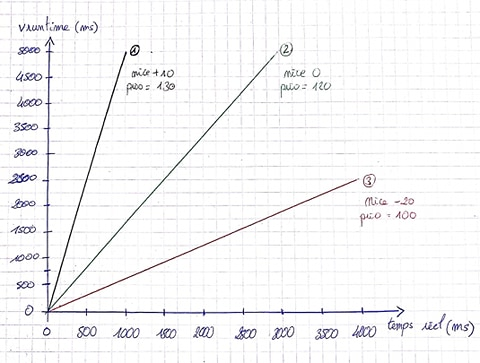
\includegraphics[scale=2.5]{include/schema_sched.jpg}
	\caption{Relation entre le vruntime et le temps réel en fonction de la priorité}
	\label{fig:sched}
\end{figure}
\\

De par ces faits nous pouvons en déduire que pour prioriser une entité, 
représentant une tâche détenant un verrou, nous pouvons influencer son 
\verb|vruntime| pour la garder à gauche de l'arbre et assurer une réélection 
rapide. Étant donné que la valeur \verb|vruntime| se base sur la priorité de 
l'entité nous avons décidé d'influencer la priorité des processus, et 
les utiliser comme un levier pour dire au scheduler de favoriser l'élection 
du processus qui détient le verrou. Pour cause, la modification du scheduler aurait
demandé d'étudier et de maîtriser tout le code et les détails du scheduler, afin
d'être sûr que nos modifications ne compromettent pas le fonctionnement de
l'ordonnanceur.

\section*{Scénario}

L'étude de scénario a été une étape importante dans notre réflexion d'optimisation de l'ordonnanceur. Cette démarche nous a permis de lever situations et cas particuliers pour la conception de notre solution.
\\

Pour simplifier, dans la suite du rapport nous considérons être sur un monoprocesseur et les tâches bloquées par le verrou sont des threads.
\\

Considérons deux tâches : un éditeur de texte (A) et un compilateur (B). La 
tâche A détient un verrou et est moins prioritaire que B. La tâche A bloque 
plusieurs autres tâches dans son exécution, elle est donc la cible de notre 
optimisation : il faut trouver un moyen de favoriser A lors des élections pour 
débloquer plus rapidement les autres tâches endormies.

Une première solution, trop naïve, était de modifier la priorité de A afin 
d'assurer sa réélection. Dans les faits, cela aurait été de modifier le 
\verb|vruntime| de l'entité correspondante afin de la placer à gauche du 
\verb|rbtree|. Comme expliqué précédemment, cela pose plusieurs problèmes, 
notamment une modification risquée du scheduler mais aussi, est-ce vraiment la 
finalité attendue ?

En forçant le placement de la tâche à gauche de l'arbre on s'assure sans 
conteste une élection au prochain tour. Cependant cela implique que la tâche 
A passe devant toutes les autres tâches, y compris la tâche B, qui est plus 
prioritaire. Cette solution écrase donc toute la logique du système de priorité 
mise en place dans le scheduler. Ce constat nous a permis d'y voir plus clair, 
nous devons trouver une solution qui garde la hiérarchie des priorités : 
favoriser A ne doit pas être un inconvénient pour B.

Une réponse à ce problème peut être d'influencer sur la priorité d'origine 
attribuée à la tâche A. Par exemple, A s'exécute avec une priorité de 120 
(valeur par défaut) et B avec une priorité de 100. On peut très bien envisager 
d'augmenter la priorité de A pour la rendre plus prioritaire sans dépasser B. 
Augmenter la priorité de 10 semble être un bon choix, A aura donc une priorité 
de 110. Cependant, dans cet exemple l'intérêt est limité, cela devient plus 
intéressant si l'on ajoute une nouvelle tâche C, de priorité 120. Les tâches A 
et C commenceront donc avec la même priorité, mais A verra sa priorité augmenter
rapidement lorsque des tâches se bloqueront sur le verrou qu'elle détient. 
Ainsi, la tâche A sera favorisée face à des tâches de priorité équivalentes mais
ne sera pas un inconvénient pour les autres tâches.

Considérons maintenant que la tâche C est semblable à la tâche A, soit un autre éditeur de texte qui bloquera elle aussi des tâches par la prise d'un verrou. Les deux tâches se verront donc voir chacune augmenter leur priorité de 10. Cependant, par la prise de son verrou, A peut peut-être bloquer plus de tâche que C, mais du point de vue du scheduler A et C sont sur un pied d'égalité en matière de priorité. De ce constat est né l'idée d'influencer la priorité de la tâche en fonction du nombre de tâches bloquées par son verrou. 
\\

On introduit donc un système de \textbf{charge}, plus une tâche a une charge élevée, plus sa priorité évolue. La priorité d'une tâche sera augmentée dans un intervalle de 0 à 10 en fonction de sa charge. Reste à établir comment calculer la charge d'une tâche. 

Une première idée aurait été de calculer cette charge avec un système de pourcentage. Un compteur qui, au fur et à mesure de la vie d'exécution de la tâche A, compterait le nombre total de tâche qui peut potentiellement se bloquer sur le verrou. Un deuxième compteur, indiquant le nombre de tâches actuellement bloquées, permettrait de calculer un pourcentage de charge. Une simple division par 10 de la charge aurait permis de calculer l'augmentation de la priorité. Mais cette solution pose le problème de garder un compteur fiable sur le nombre de tâches pouvant potentiellement se bloquer sur le verrou. De plus le pourcentage de charge n'est pas très parlant. Imaginons que A et C ont toutes les deux une charge de 100\% mais A bloque 100 tâches contre 10 pour C. Bien que A devrait être plus favorisé il n'en reste que A et C auront toutes les deux une priorité augmentée de 10.
\\

Plutôt que de se perdre dans de lourds calculs de charge avec des pourcentages, nous avons décidé de s'orienter vers une implémentation plus simple. La charge correspondra au nombre total de tâches couramment bloquées sur le verrou. Ainsi, la priorité ajoutée à la tâche propriétaire du verrou restera toujours dans un intervalle de 0 à 10 mais fonctionnera par paliers : sur des échelons restant encore à définir, on peut envisager que toutes les 5 tâches bloquées la priorité se voit augmenter de 1, plafonnant ainsi l'augmentation à 50 tâches bloquées.
\\

Pour rendre cette implémentation plus efficace nous ajoutons le
mécanisme d'héritage de priorité. Considérons pour simplifier deux fils d'exécution
(tâche 1 et 3) qui partagent le même espace d'adressage et qui veulent accéder à une même section critique, et un processus (tâche 2) qui contient un seul fil d'exécution indépendant des deux 
premiers, dont les priorités sont définies comme ceci: Pri(3) $>$ Pri(2) $>$ 
Pri(1), même en considérant l'augmentation de priorité définie précédemment.
\\

NB: cette configuration peut être aussi atteignable avec 3 processus dont deux 
utilisent un segment de mémoire partagé ou bien 3 threads d'un même processus.
\\

Si la tâche 1, qui se trouve être la moins prioritaire, prend un futex et que 
la tâche 3, qui est la plus prioritaire, veut aussi l'acquérir, elle
devra se bloquer en attendant que la tache 1 libère le verrou. Étant donné que la tâche 2 possède une priorité plus élevée que le propriétaire du futex, elle sera choisie plus fréquemment par le scheduler. Ce comportement va ralentir l'exécution de la tâche 3, la plus prioritaire, qui est bloquée en attente de la libération du futex par la tâche 1.

\begin{figure}[h!]
	\centering
	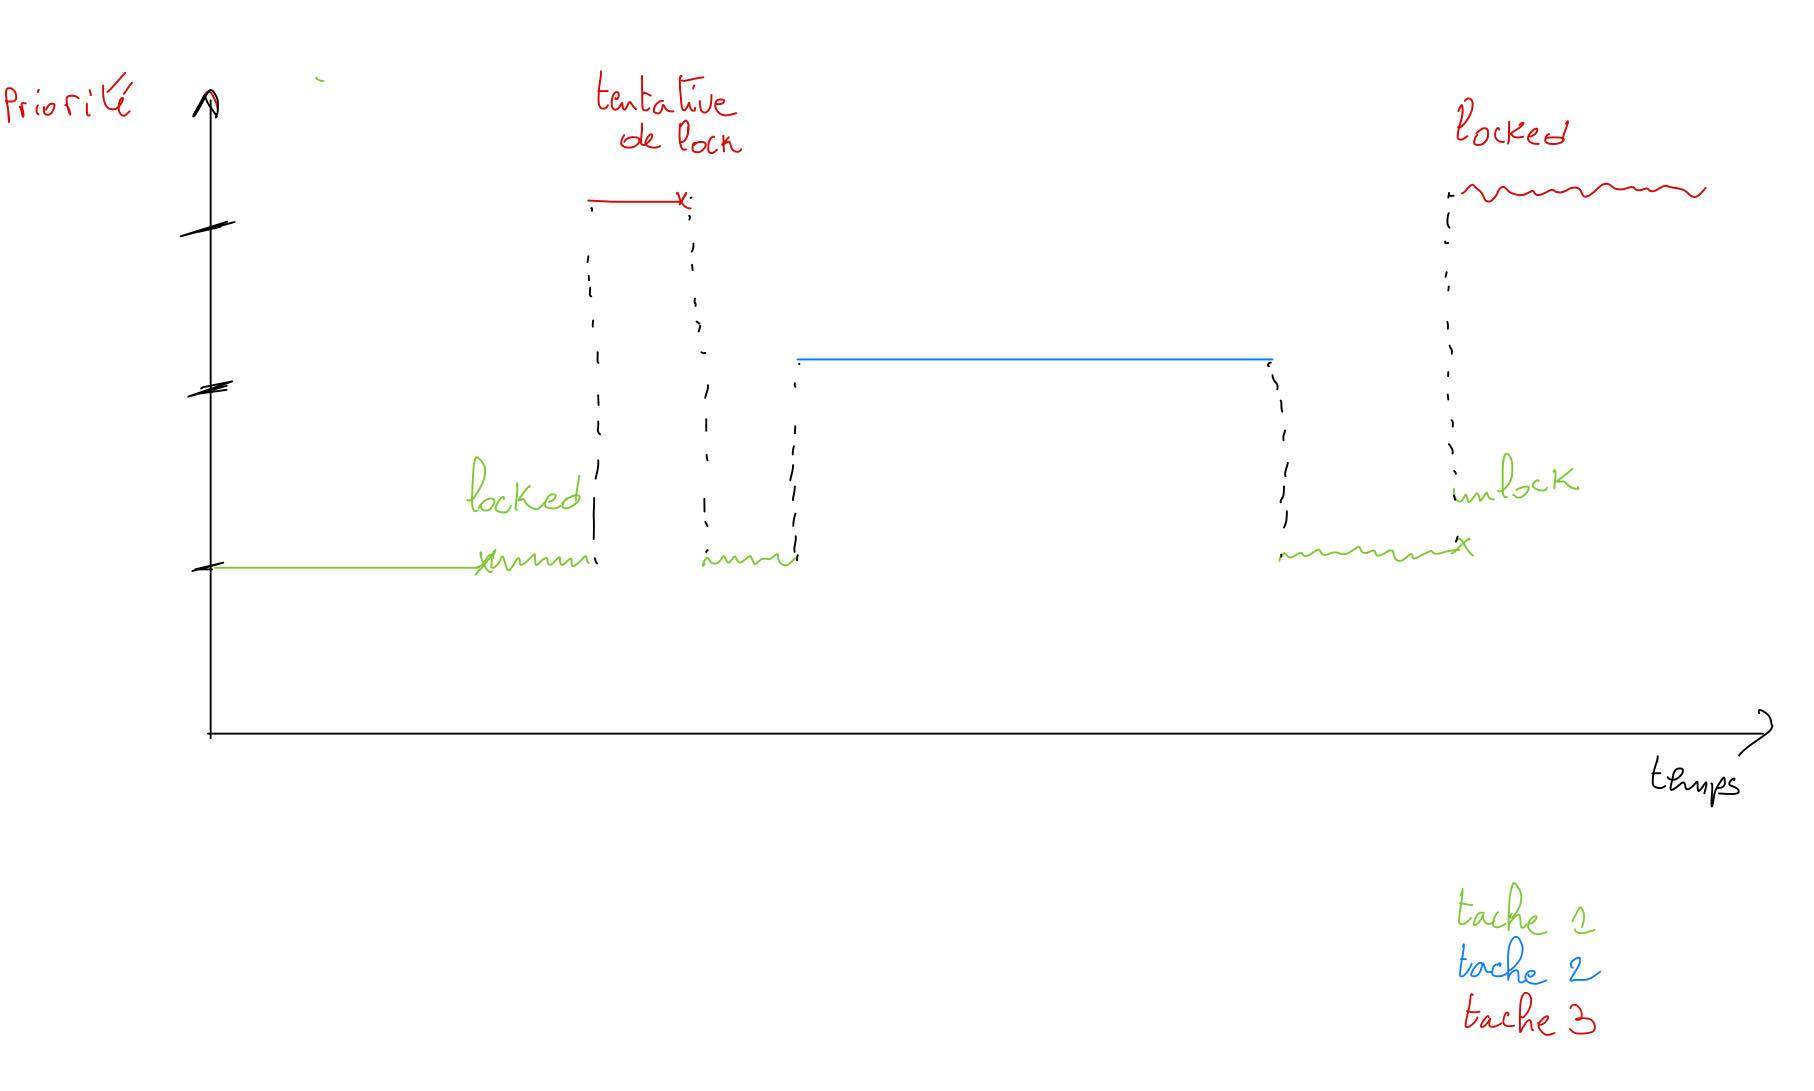
\includegraphics[scale=0.21]{include/without_inherit.jpg}
	\caption{Avancement des processus sans l'heritage de priorité}
	\label{fig:without_inherit}
\end{figure}

\newpage


L'idée ici est de modifier la priorité de la tâche 1 pour qu'elle soit plus 
prioritaire que la tâche 2. On peut atteindre cela en héritant de la 
priorité de la tâche 3, qui est plus prioritaire que la tâche 2. 

Ainsi, le propriétaire du verrou se verra attribuer, au cours de son exécution, la priorité de la tâche la plus prioritaire parmi toutes les tâches bloquées sur le verrou. De plus, l'augmentation de la priorité par rapport à la charge introduite précédemment sera appliquée à cette nouvelle priorité.

\begin{figure}[h!]
	\centering
	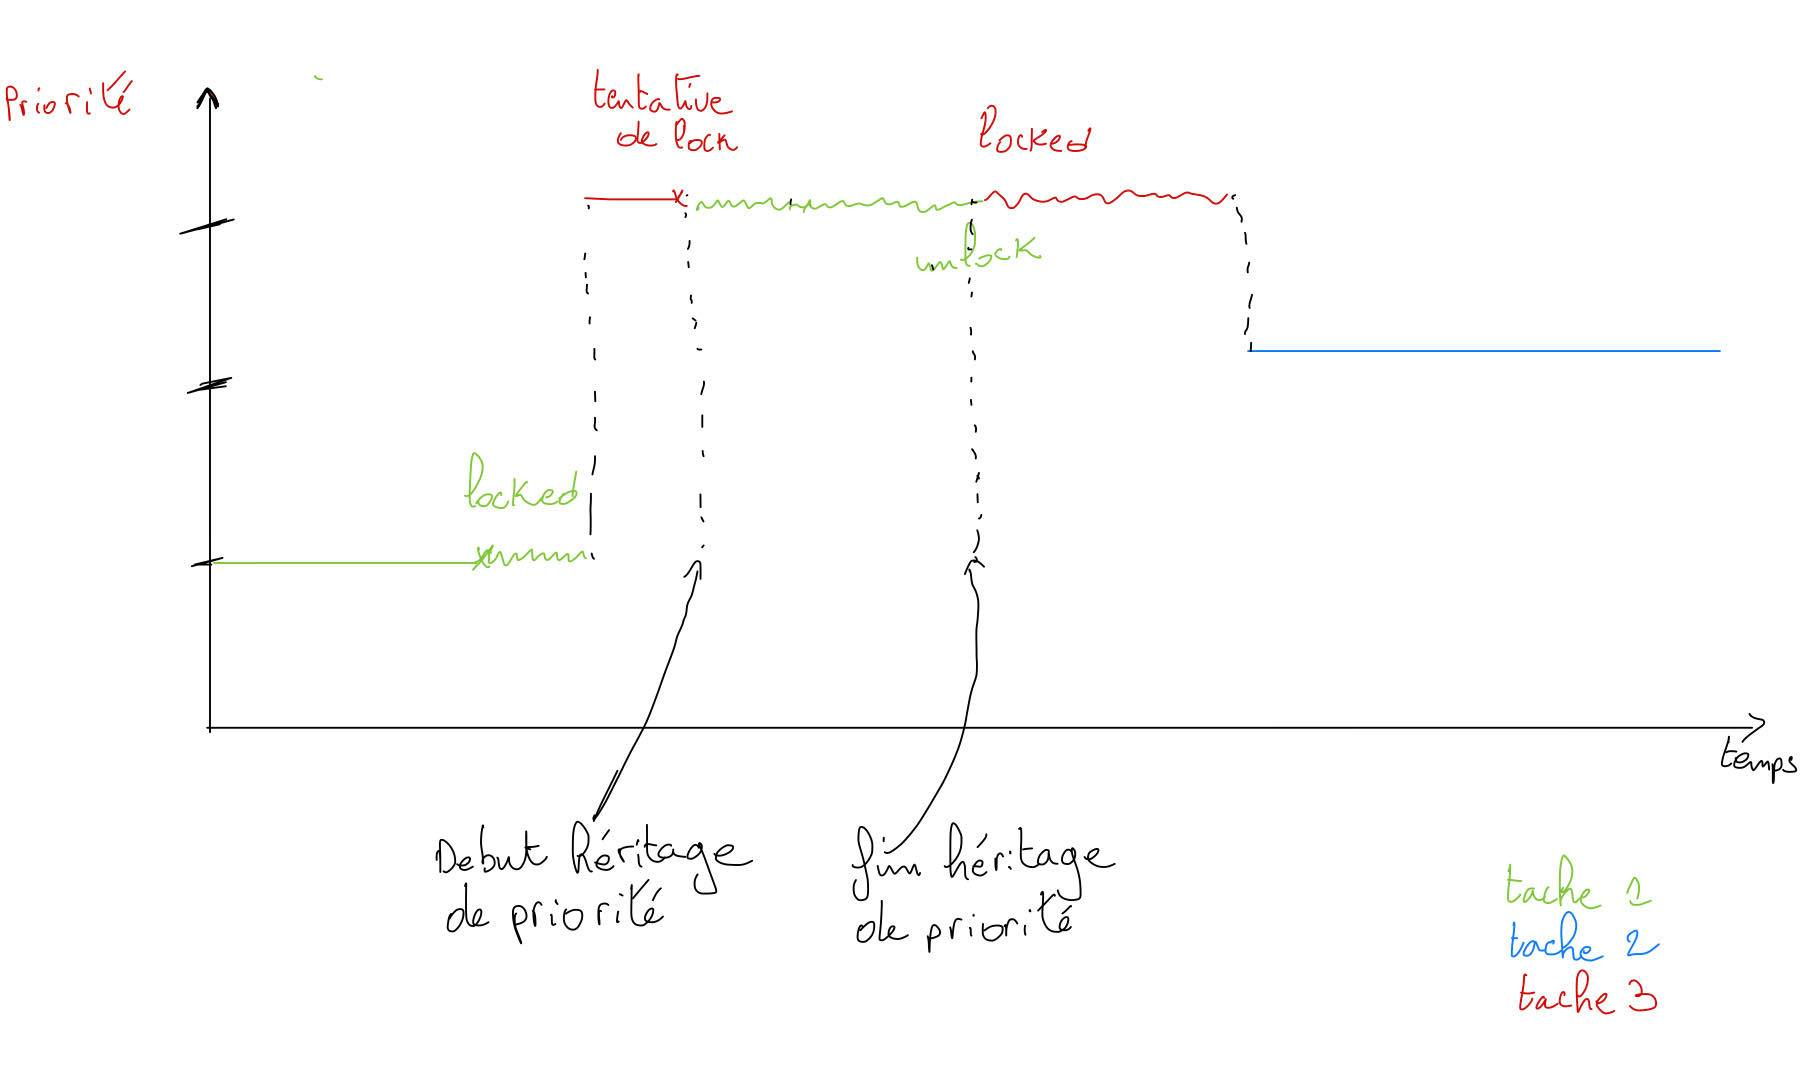
\includegraphics[scale=0.21]{include/with_inherit.jpg}
	\caption{Avancement des processus avec l'heritage de priorité}
	\label{fig:with_inherit}
\end{figure}

Le CFS est connu pour être un scheduler très équitable, en combinant ces deux techniques cela permet d'assurer une implémentation qui reste juste pour chaque tâche.

\section{Implémentation}

Notre choix d'implémentation a donc été de ne pas modifier directement le code du scheduler (\verb|<kernel/sched/fair.c>|), mais d'ajouter notre mécanisme lors de la prise de
verrou dans le code
du futex (\verb|<kernel/futex.c>|) et d'agir directement sur les priorités des tâches.

L'ensemble de nos modifications dans le kernel on été préfixé par un commentaire \verb|MAS code|.

\subsection{Structure}

La première étape à donc été de créer un mécanisme permettant au kernel de pouvoir facilement
suivre l'évolution du propriétaire d'un futex.
Nous avons donc ajouté une structure \verb|futex_state| qui représente l'état d'un
futex:

\begin{lstlisting}[tabsize=4]
struct futex_state {
	struct list_head list;
	struct task_struct *owner;
	raw_spinlock_t spin_lock;
	struct kref refcount;
	int load;
	union futex_key *key;
};
\end{lstlisting}

Les champs sont les suivants:
\begin{itemize}
	\item \verb|list| permet de créer un chaînage entre les futex d'un même propriétaire.
	
	\item \verb|owner| est une référence sur la \verb|task_struct| du propriétaire du futex.
	
	\item \verb|spin_lock| permet d'éviter les accès concurrents lors de la manipulation de
	la structure.
	
	\item \verb|kref| est un compteur de référence pour protéger la suppression
	des structures, et ainsi éviter de libérer la structure utilisée ailleurs.
	
	\item \verb|load| est le poids associé au futex.
	
	\item \verb|key| est la clé du futex, permettant d'identifier la structure pour un 
	futex donné.
\end{itemize}
\hspace{1cm}

Une modification sur la structure \verb|task_struct| a été nécessaire:

\begin{lstlisting}[tabsize=4]
struct task_struct {
	...
	struct list_head futex_state_list;
	raw_spinlock_t futex_state_lock;
	struct futex_state *waiting_futex_state;
	int user_nice;
	int futex_state_prio;
	...
}
\end{lstlisting}

Les champs ajoutés sont les suivants:
\begin{itemize}
	\item \verb|futex_state_list| est l'ensemble des
	\verb|futex_state| que la tâche détient et sur lesquels d'autres tâches attendent.
	
	\item \verb|futex_state_lock| est un verrou pour la manipulation de la liste.
	
	\item \verb|waiting_futex_state| est un pointeur vers le \verb|futex_state| sur lequel
	la tâche attend.
	
	\item \verb|user_nice| est le valeur courante du nice utilisateur appliquée à la tâche.
	
	\item \verb|futex_state_prio| est l'augmentation de priorité appliquée à la tâche en fonction
	des autres tâches qu'elles bloquent.
\end{itemize}

\subsection{Fonctionnement}

Lorsqu'une tâche souhaite prendre un verrou déjà détenu elle passe en mode kernel. 
C'est là que notre mécanisme rentre en jeu.

L'appel système place dans \verb|uaddr| l'adresse du verrou côté user. 
La valeur du verrou, contenant le pid du propriétaire, peut être récupérée avec \verb|get_user(uval, uaddr)|.
Ainsi, la tâche qui va se bloquer en attente du verrou connaît le pid du propriétaire avec une simple
opération bit à bit sur \verb|uval| et peut accéder sa structure \verb|task_struct| avec
\verb|find_task_by_vpid(vpid)|.

\subsubsection{Prise de verrou}

Lors de la prise de verrou notre première étape est de récupérer la \verb|futex_key| 
associé au futex sur lequel la tâche va se bloquer:
\begin{lstlisting}[tabsize=4]
	get_futex_key(uaddr, 0, key, VERIFY_READ);
\end{lstlisting}
Ensuite il faut récupérer le \verb|futex_state| associé à cette \verb|futex_key|:
\begin{lstlisting}[tabsize=4]
	get_futex_state(owner, key, &state);
\end{lstlisting}

Cette fonction va regarder si le \verb|futex_state| associé à la clé \verb|key| existe
dans la liste du \verb|owner|,
si la structure n'existe pas alors elle sera allouée, initialisée et ajoutée à la liste du \verb|owner|,
sinon elle sera retournée.
Dans les deux cas le compteur de référence du \verb|state| retourné sera incrémenté.

Pour indiquer que la tâche courante va s'endormir en attendant sur le futex, on passe la structure
du \verb|futex_state| précédemment récupérée à la \verb|task_struct|:
\begin{lstlisting}[tabsize=4]
	current->waiting_futex_state = state;
\end{lstlisting}

\subsubsection{Héritage de charge}

Après l'ajout de la tâche courante comme tâche en attente du futex il faut appliquer le changement de charge
par héritage:
\begin{lstlisting}[tabsize=4]
	futex_state_inherit(current, state, 
						FUTEX_STATE_LOAD);
\end{lstlisting}

La tâche courante \verb|current| peut elle aussi bloquer plusieurs tâches sur plusieurs verrous, ainsi il est important de ne pas
simplement incrémenter de 1 le poids du futex sur lequel on va attendre, mais de la somme des poids
des \verb|futex_state| que la tâche courante détient. Cette somme est calculée avec un simple parcourt sur la
liste des \verb|futex_state| de la tâche:
\begin{lstlisting}[tabsize=4]
	get_futex_state_sumload(task);
\end{lstlisting}

Le propriétaire de \verb|state| peut lui aussi attendre sur un \verb|futex_state|,
détecté grâce au champs \verb|waiting_futex_state|. 
Le principe d'héritage demande donc
de procéder par récurrence sur l'arbre et de mettre à jour le poids de chaque \verb|futex_state|
et ainsi remonter à la tâche qui n'attend pas sur un verrou, le \textit{master futex owner}.
C'est ce dernier qui verra sa priorité changer à partir de son poids.

\begin{lstlisting}[tabsize=4]
int futex_state_inherit(struct task_struct *task, 
						struct futex_state *state,
						int op)
{
	struct futex_state *m_state;
	int sumload;
	
	if (op != FUTEX_STATE_LOAD && 
		op != FUTEX_STATE_UNLOAD)
		return -1;
	
	/* Recupere la somme des poids des eventuelles 
 	   futex_state que l'on detient */
	sumload = get_futex_state_sumload(task);
	
	/* Remonte l'arbre jusqu'au master futex 
 	   owner et applique le poids a chaque futex_state */
	do {
		m_state = state;
		state->load += (sumload + 1) * op;
	} while ((state = state->owner->waiting_futex_state)
		!= NULL);
	
	/* Applique la priorite sur le master futex owner */
	futex_state_prio(m_state->owner);
	
	return 0;
}
\end{lstlisting}

\subsubsection{Application de la priorité}

La fonction \verb|futex_state_prio(task)| permet de définir la priorité d'une tâche en se
basant sur son \verb|sumload|. L'implémentation finale est très simple et peut être la cible
d'amélioration. 
\begin{lstlisting}[tabsize=4]
void futex_state_prio(struct task_struct *task)
{
	int load = get_futex_state_sumload(task);
	
	if (load < 0)
		load = 0;
	
	if (load > FUTEX_STATE_MAX_PRIO)
		load = FUTEX_STATE_MAX_PRIO;
	
	task->futex_state_prio = load;
	set_static_prio(task);
}
\end{lstlisting}

L'augmentation attribuée à la tâche correspond au nombre de tâche qu'elle bloque, borné sur 
\verb|FUTEX_STATE_MAX_PRIO| valant 20.

La fonction \verb|set_static_prio(task)| est ensuite appelé.
Cette fonction se situe dans \verb|<kernel/sched/core.c>| et permet de modifier la priorité
statique d'une tâche en combinant le nice utilisateur (\verb|user_nice|) et l'augmentation
de priorité lié au futex state (\verb|futex_state_prio|).
Voici son code simplifié:

\begin{lstlisting}[tabsize=4]
void set_static_prio(struct task_struct *p)
{
	int prio;
	
	prio = NICE_TO_PRIO(p->user_nice) - p->futex_state_prio;
	
	...
	
	p->static_prio = prio;
	set_load_weight(p, true);
	old_prio = p->prio;
	p->prio = effective_prio(p);
	
	...
}
\end{lstlisting}

La fonction appelée lors de la modification du nice par l'utilisateur a aussi
subi des changements:
\begin{lstlisting}[tabsize=4]
void set_user_nice(struct task_struct *p, long nice)
{
	if (task_nice(p) == nice || nice < MIN_NICE 
		|| nice > MAX_NICE)
	return;
	
	p->user_nice = nice;
	set_static_prio(p);
}
\end{lstlisting} 

Ce mécanisme de changement de priorité permet de faire cohabiter le nice utilisateur
et l'augmentation de priorité des \verb|futex_state|.
Quand l'une des deux valeurs change l'autre est toujours prise en compte.
On peut donc voir la variable \verb|futex_state_prio| comme un offset qui décale la priorité de base
(\verb|DEFAULT_PRIO| = 120) sur lequel le nice base son calcul.



\subsubsection{Changement de propriétaire}

Lorsqu'une tâche détenant un verrou le relâche, celui-ci réveille toutes les autres tâches en attente
du verrou. La tâche qui sera le nouveau propriétaire le déclare avec la fonction:
\begin{lstlisting}[tabsize=4]
	fixup_state_owner_current(state);
\end{lstlisting}
Cette fonction va notamment modifier le \verb|owner| de \verb|state|, décrémenter son poids, ajouter 
le \verb|state| à sa liste, et ainsi pouvoir appliquer sa priorité basé sur ces changements avec
\verb|futex_state_prio(task)|. Le champs \newline \verb|waiting_futex_state| de la tâche courante est marqué à \verb|NULL|
pour indiquer que celle-ci n'attend plus sur un futex. Voici le code de la fonction:

\begin{lstlisting}[tabsize=4]
int fixup_state_owner_current(struct futex_state *state)
{
	int sumload = get_futex_state_sumload(current);
	state->owner = current;
	add_futex_state(state);

	state->load -= (sumload + 1);	

	futex_state_prio(state->owner);
	
	kref_put(&state->refcount, free_futex_state);
	current->waiting_futex_state = NULL;
	
	return 0;
}
\end{lstlisting}

Il faut noter que le poids est décrémenté de 1 plus la somme des poids des \verb|futex_state| 
que le nouveau propriétaire détient avant l'ajout du \verb|state|. En effet, en se bloquant on a hérité notre \verb|sumload| au \verb|state|, en devenant son propriétaire il faut donc déshériter ce même \verb|sumload|.

\subsubsection{Relâchement d'un verrou}

Lors du relâchement d'un verrou la tâche courante, le propriétaire, doit récupérer le \verb|futex_state| associé:
\begin{lstlisting}[tabsize=4]
	fetch_futex_state(current, key, &state);
\end{lstlisting}
Si le \verb|state| existe alors il est retiré de la liste:
\begin{lstlisting}[tabsize=4]
	del_futex_state(state);
\end{lstlisting}
Après ces changements la priorité de la tâche courante doit être mis à jour:
\begin{lstlisting}[tabsize=4]
	futex_state_prio(current);
\end{lstlisting}

Ainsi, si la tâche relâche son dernier verrou alors sa liste devient vide et l'appel
à \verb|futex_state_prio(task)| annulera les modifications de priorité apportées.

\subsubsection{Mort subite}

Il se peut qu'un processus meurt alors qu'il attend sur un verrou. De la même manière que lors de
l'attente sur un verrou, il faut cette fois-ci décrémenter par récurrence sur l'arbre 
le poids des \verb|futex_state|.
Une modification de la fonction \verb|do_exit| dans \verb|<kernel/exit.c>| a donc été nécessaire:
\begin{lstlisting}[tabsize=4]
if (tsk->waiting_futex_state != NULL) {
	futex_state_inherit(tsk, tsk->waiting_futex_state,
						FUTEX_STATE_UNLOAD);
	kref_put(&tsk->waiting_futex_state->refcount, 
			free_futex_state);
}
\end{lstlisting}

Si la tâche courante attend sur un futex on applique donc un deshéritage et on relâche la référence sur le
\verb|futex_state|. 

\subsection{Shrinker}

Les shrinker permettent une optimisation mémoire.
Dans notre cas leur utilisation n'est pas possible. En effet, on ne peut pas se permettre 
de supprimer ou bien de libérer une référence d'une structure \verb|futex_state| en cours 
d'utilisation, cela peut compromettre tout le mécanisme de verrouillage des futex.

\section{Benchmark}

Pour évaluer notre implémentation nous avons réalisé un petit benchmark qui se charge de simuler un
scénario basique.

\noindent \textbf{Scénario:}
Un thread parent prend un mutex et lance l'exécution de 20 threads enfant se bloquant sur son mutex.
Une fois les enfants lancés, le parent exécute son calcul.
10 autres threads s'exécutent en parallèle du thread parent et effectue leur calcul.
Le programme s'arrête brutalement quand le parent a fini l'exécution de son calcul.

\noindent \textbf{Calcul des threads:} 
Calcul du déterminent d'une matrice 11x11.

\noindent \textbf{Résultat attendu:}
Les 20 threads enfant doivent augmenter la priorité du thread parent de 20,
jouant donc comme un nice -20. Le thread parent doit donc voir son temps d'exécution significativement
réduit et finir avant les threads parallèles.

\noindent \textbf{Environnement de test:}
Machine virtuelle avec 1 cœur.

\noindent \textbf{Résultat:}
Temps d'exécution \textbf{sans} notre implémentation des futex state:
\begin{lstlisting}
real	0m43.359s
user	0m43.326s
sys	0m0.011s
\end{lstlisting}
Le thread parent ne fini pas avant les threads parallèles.

\noindent Temps d'exécution \textbf{avec} notre implémentation des futex state:
\begin{lstlisting}
real	0m4.406s
user	0m4.396s
sys	0m0.003s
\end{lstlisting}
Le thread parent fini bien avant les threads parallèles.

Par manque de temps nous n'avons pas pu évaluer notre implémentation sur des scénarios plus complexes,
notamment en jouant avec le multicœur. 

\section{Discussion}

Nous concluons ce projet par un bilan sur sa réalisation et ses résultats ainsi qu'une discussion sur 
ses limites et les améliorations envisageables.

\subsection{Réalisation du projet et limite}

La réalisation du projet s'est bien déroulé, toutes les fonctionnalités attendues on été
implémentées.
Les résultats sur l'évaluation de notre mécanisme sont globalement concluant, bien que 
par manque de temps nous aurions préféré affiner nos benchmarks.

Cependant le projet a montré des limites, notamment sur la manipulation de la liste \verb|futex_state_list| d'une tâche.
Son utilisation requière la prise du verrou \verb|futex_state_lock|.
Ainsi, lors de la recherche, d'un ajout ou d'une suppression d'un \verb|futex_state|
sur la liste mais aussi lors du calcul de la somme, le verrou est pris. Cela empêche d'autres tâches bloquées
sur la même tâche propriétaire d'y accéder. Créant ainsi des groupes de tâches à cette prise de
verrou commun. Il y a donc un risque de contention entre ces tâches.

Dans les premières implémentations nous avions créé un liste globale, recensant l'ensemble des \verb|futex_state| quelque soit
leur propriétaire. Sa manipulation était donc commune à toutes les tâches, en plus du manque de performance de 
cette méthode, le problème de contention était d'autant plus présent. L'utilisation des listes, dites locales, à chaque
propriétaire permet de réduire ce problème de contention. Cependant le risque persiste et aucune solution 
viable nous semble contourner ce problème pour le moment.

\subsection{Travaux à court terme}
Par manque de temps certaines tâches n'ont pas pu être réalisées dans le temps imparti.
Leur implémentation n'ont pas d'impact majeur et elles ont donc été laissé pour les travaux à court terme.

\subsubsection{Poids}
La clé de voûte de notre implémentation est son système de poids.
Lors de l'héritage nous avons vu que la tâche qui va se bloquer doit calculer la somme
des poids des \verb|futex_state| qu'elle détient, représenté ensuite par une variable \verb|sumload|.
Ce calcul est effectué plusieurs fois, et demande de parcourir la liste des \verb|futex_state| de la tâche.
Or, nous pouvons réduire ces calculs par un champs dans la structure \verb|task_struct| qui représenterai
la valeur \verb|sumload| à tout instant. Cette variable serait mis à jour lors de l'héritage, deshéritage,
ajout et suppression de \verb|futex_state|.

\subsubsection{Généralisation}
Par manque de temps l'implémentation n'a été qu'effectué que pour l'utilisation des mutex de type PI 
(héritage de priorité). Un travail à court terme serait de le rendre
fonctionnel pour l'utilisation des mutex de type ROBUST, soit le protocole par défaut.

Cette décision est une question de débogage, nous permettant 
de tester notre implémentation volontairement avec des programmes tests en utilisant
des mutex PI. En effet, en implémentant le mécanisme, en cours de développement,
 pour le type ROBUST le kernel l'aurait utilisé, ce qui aurait compliqué le débogage lors d'éventuelles erreurs.

\subsection{Travaux à long terme: les priorités}
L'implémentation actuelle du changement de priorité d'une tâche par la fonction \verb|futex_state_prio(task)| 
est très simpliste. Elle réside en une réduction de la \verb|static_prio| par le \verb|sumload| 
borné sur 20.

Pour rendre plus juste la modification de la priorité nous pouvons envisager l'utilisation d'une formule.
Une approche peut consister à attribuer un coefficient à chaque tâche bloquée. 
Ce coefficient est calculé en fonction de la priorité de la tâche. 
Plus la tâche est prioritaire et plus son coefficient est élevé.
Le poids qu'ajoutera la tâche bloquée au \verb|futex_state| du propriétaire dépendra de son coefficient.
Ainsi par exemple, une tâche de priorité 120 ajoutera 1 au poids, tandis qu'une tâche de priorité 100
ajoutera 2. 

Ce système permet d'être encore plus équitable entre les tâches. Deux tâches de même priorité bloquant
le même nombre de tâches auront un \verb|sumload| différent en fonction des priorités des tâches qu'elles bloquent.

Cette nouvelle approche complexifie le mécanisme, notamment si une tâche bloquée voit sa priorité modifiée
lorsqu'elle dort, son coefficient devra être mis à jour en conséquent.



%\include{conclusion}

%\include{annexe}
\clearpage

%\bibliographystyle{plain}
%\bibliography{bibliography}

\end{document}
